\section{Unfolding}
%%%%%%%%%%%%%%%%%%%%%%%%%%%%%%%%%%%%%%%%%%%%%%%%%%%%%%%%%%%%%%%%%%%%%%
\label{sec:Unfolding}

To facilitate comparisons with theoretical predictions or other experimental results, the signal
extracted performing the fit has to be corrected for detector resolution and
efficiency effects and for the efficiency of the selection defined in the
analysis.
An unfolding procedure is used relying on the \textsc{RooUnfold} package
\cite{Adye:2011gm}, which provides the tools to run various unfolding
algorithms.

The basic principle behind the unfolding procedure in this analysis is to use MC signal samples
to make the ``true'' distribution of the variable of interest, which is obtained using simulated events before particle interaction with the detector, and the same distribution obtained
using events reconstructed after the full \textsc{Geant4} simulation of the CMS detector
and event reconstruction. These two distributions are used to calculate the detector
response matrix $M$:

\begin{equation}\label{eq:resp_matrix}
R_{i}^{\rm {MC}} = \sum_{j=1}^{n} M_{ij}T_{j}^{\rm {MC}} \quad ,
\end{equation}

where $R^{\rm{MC}}$ and $T^{\rm{MC}}$ are two $n$-dimensional vectors
representing the distribution before and after event processing through CMS
simulation and reconstruction. The dimension $n$ of the two vectors corresponds 
to the number of bins in the distributions, equal to six in this analysis.
The response matrix $M$ includes all the effects related to the detector and analysis selection that affect the $R^{\rm{MC}}$ distribution.
The goal of the unfolding procedure is to obtain the $T^{\rm{truth}}$ distribution starting from the measured
$R^{\rm{observed}}$ distribution by inverting the matrix $M$.
To avoid the large variance and strong negative correlation between the neighbouring bins~\cite{Cowan:2002in}, the unfolding procedure in this analysis relies on the singular value decomposition~\cite{Hocker:1995kb} method based on the Tikhonov regularization
function.
Since the response matrix is in general limited by the statistical uncertainties of simulated samples and given the finite data statistical accuracy, a simple inversion could lead to large fluctuations between bins in the unfolded result. In particular, if the off-diagonal elements
of the response matrix are sizeable, the unfolded distribution has large variance and 
strong negative correlations between the neighbouring bins~\cite{Cowan:2002in}.
Several unfolding methods with regularization are available in literature, such as a method based on the Bayes' theorem, which overcome 
the unfolding instability using an iterative procedure~\cite{D'Agostini:1994zf}.
One possible solution is the utilization of regularization methods.
Such methods introduce a regularization function that controls the smoothness of the distribution 
and depends generally on one regularization parameter, which can be controlled
to achieve the desired degree of smoothness.
The choice of the regularization parameter is particularly critical, and it
should represent an optimal trade-off between taming the fluctuations in the
unfolded result, and biasing the unfolded distribution towards the one used to
build the response matrix. 
The principle feature of this method is the use of the singular value decomposition of the response matrix, including an additional term to suppress the oscillatory component of the solution, i.e. the regularization term, which represents some \textit{a priori} knowledge of the final solution.
The regularization parameter is chosen to obtain results that are robust against numerical instabilities and statistical fluctuations, following the prescription described in Ref.~\cite{Hocker:1995kb}.
It has been verified using a large number of simulated pseudo-experiments that the coverage of the unfolded uncertainties obtained with this procedure is as expected.

The response matrix is built as a two-dimensional histogram, with the
generator-level \pth{} on the $y$ axis and the same variable after the reconstruction on the $x$ axis, using the same binning for both
distributions.
The resulting detector response matrix, including all signal sources and normalized by row, is shown in Fig.~\ref{fig:matrix}(a).
The value of the diagonal bins corresponds to the stability S. The same matrix, normalized by column, is shown in Fig.~\ref{fig:matrix}(b). In this case the diagonal bins correspond to the purity P. The $S$ and $P$ parameters, defined in Sec.~\ref{sec:AnalysisStrategy}, provide an estimate of the \pth resolution and migration effects.
The main source of bin migrations effects in the response matrix is the limited resolution in the measurement of \MET.

The resulting detector response matrix, which includes the effects of all signal sources and is represented by normalizing each row to unity is shown in Fig.~\ref{fig:matrix}(a). This representation shows the stability $S$ in the diagonal bins, where $S$ is defined as the ratio of the number of events generated and reconstructed in a given bin, and the number of events generated in that bin. In addition, a deconvolution matrix is constructed by normalizing each column to unity and is shown in Fig.~\ref{fig:matrix}(b). This latter representation shows the purity $P$ in the diagonal bins, where $P$ is defined as the ratio of the number of events generated and reconstructed in a given bin, and the number of events reconstructed in that bin. The $S$ and $P$ parameters provide an estimate of the \pth{} resolution and of migration effects.
The response matrix built including all signal sources is shown in Fig.~\ref{fig:matrix}. In order to point out either the purity or the stability in diagonal bins, each column or row of the matrix was respectively normalized to unity. The matrix obtained in the first case is what is actually called detector response matrix, while in the other case the matrix is usually referred to as detector deconvolution matrix.

\begin{figure}[!h]
\centering
\subfigure[Response matrix]{
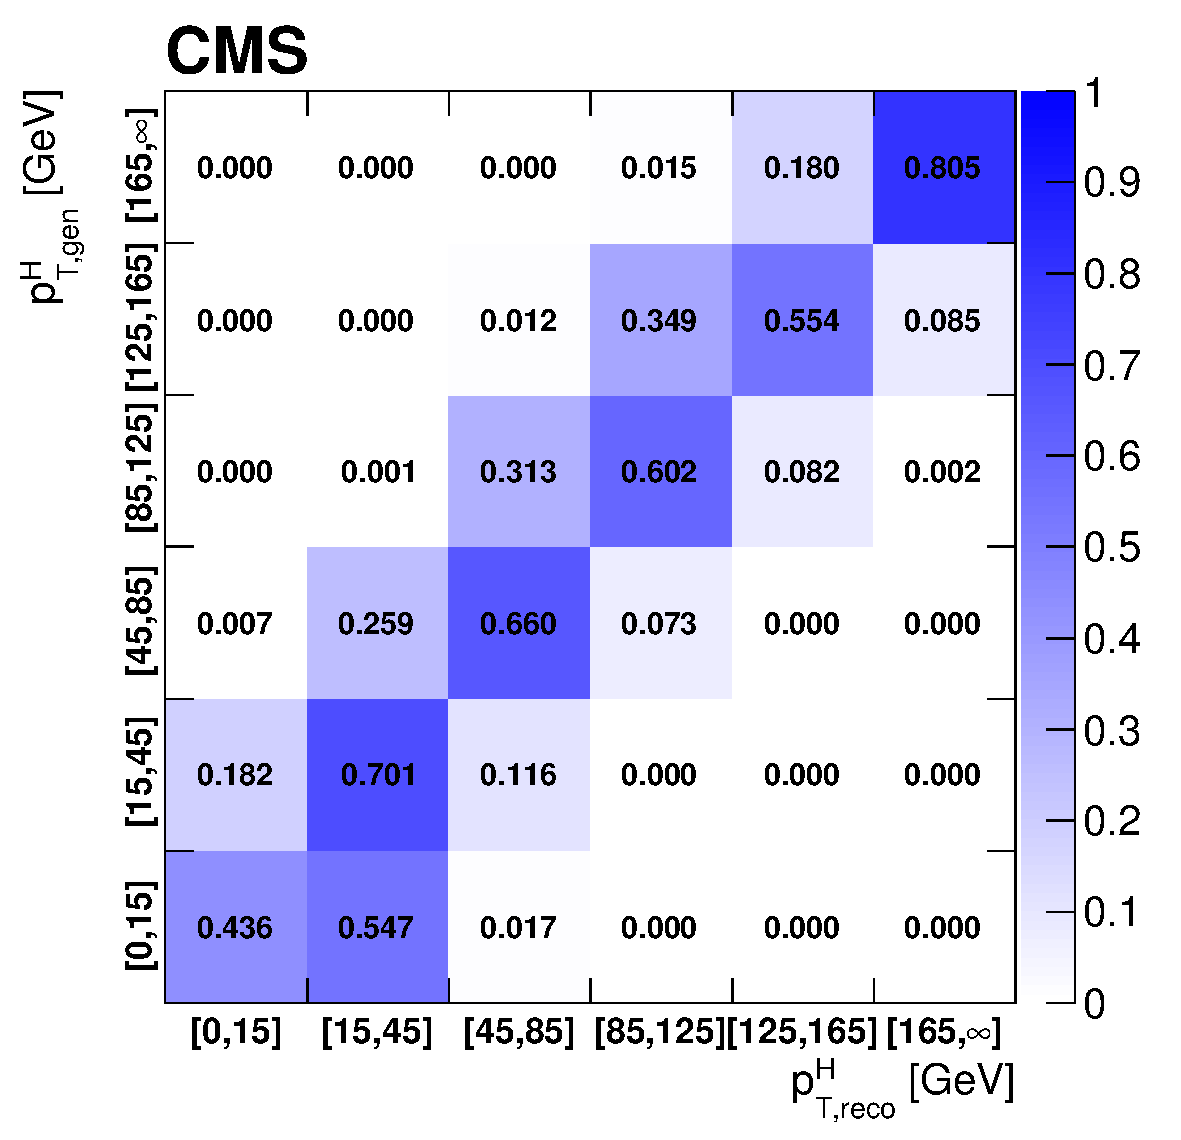
\includegraphics[width=0.5\textwidth]{images/matrix_byrow_paper.pdf}
}
\subfigure[Deconvolution matrix]{
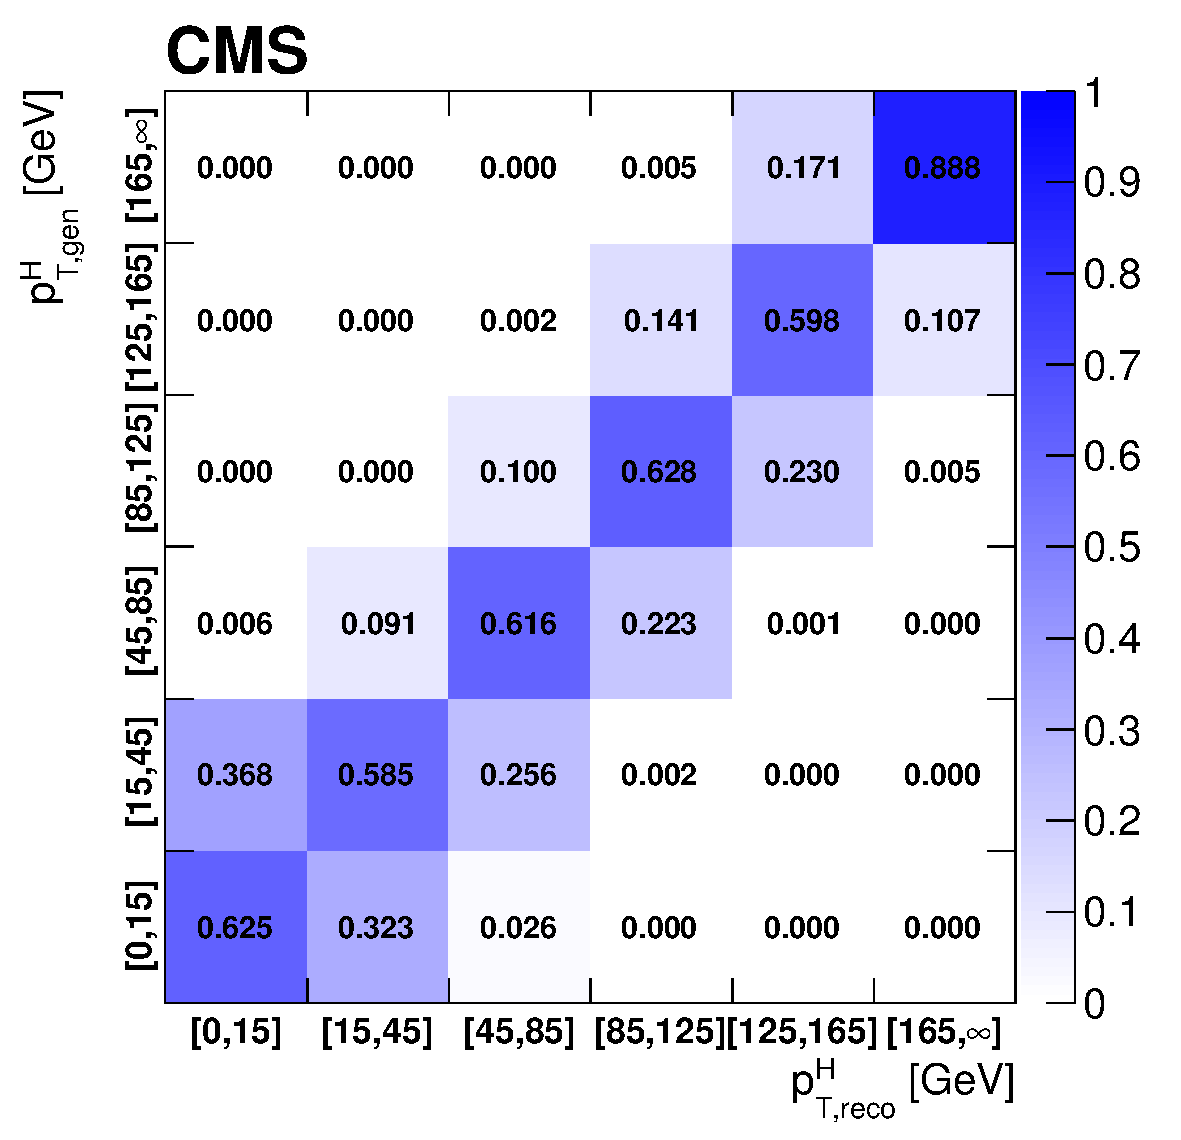
\includegraphics[width=0.5\textwidth]{images/matrix_bycol_paper.pdf}
}
\caption{Response matrix (a) and deconvolution matrix (b) including all signal processes. The matrices are normalized either by row (a) or by column (b) in order to show the purity or stability respectively in diagonal bins.}\label{fig:matrix}
\end{figure}

Several closure tests are performed in order to validate the unfolding
procedure. To estimate the uncertainty in the unfolding procedure due to the
particular model adopted for building the response matrix, two independent
gluon fusion samples are used, corresponding to two different generators:
\textsc{Powheg V1} and \textsc{JHUGen} generators, both interfaced to \textsc{Pythia 6.4}.
The \textsc{JHUGen} generator sample is used to build the response matrix while the
\textsc{Powheg V1} sample is used for the measured and the MC distributions at
generator level. The result of this test shows good agreement between the unfolded and the distribution from MC simulation.




























\textcolor{red}{Adjust the following part}




In order to show the unfolded spectrum dependence on the choice of the regularization parameter, the unfolded procedure has been repeated for several regularization values. The various plots are shown in figure \ref{fig:kreg_test} for regularization values varying from 1 (stronger regularization) to 5 (weaker regularization). Using $k_{reg} = 6$ is equivalent to the simple inversion of the response matrix and leads to huge errors. Lowering $k_{reg}$ means increasing the regularization and thus reducing the statistical uncertainty. One should increase the regularization as much as possible until the procedure starts to bias the distribution. The distribution starts to be biased, according to the $\log{d_i}$ curve criterion, at $k_{reg} = 2$. Looking at figure \ref{fig:kreg_test}, the bias is clearly visible especially for $k_{reg} = 1$, when the unfolded distribution does not match anymore the MC truth.

\begin{figure}[htb]
\centering
\subfigure{
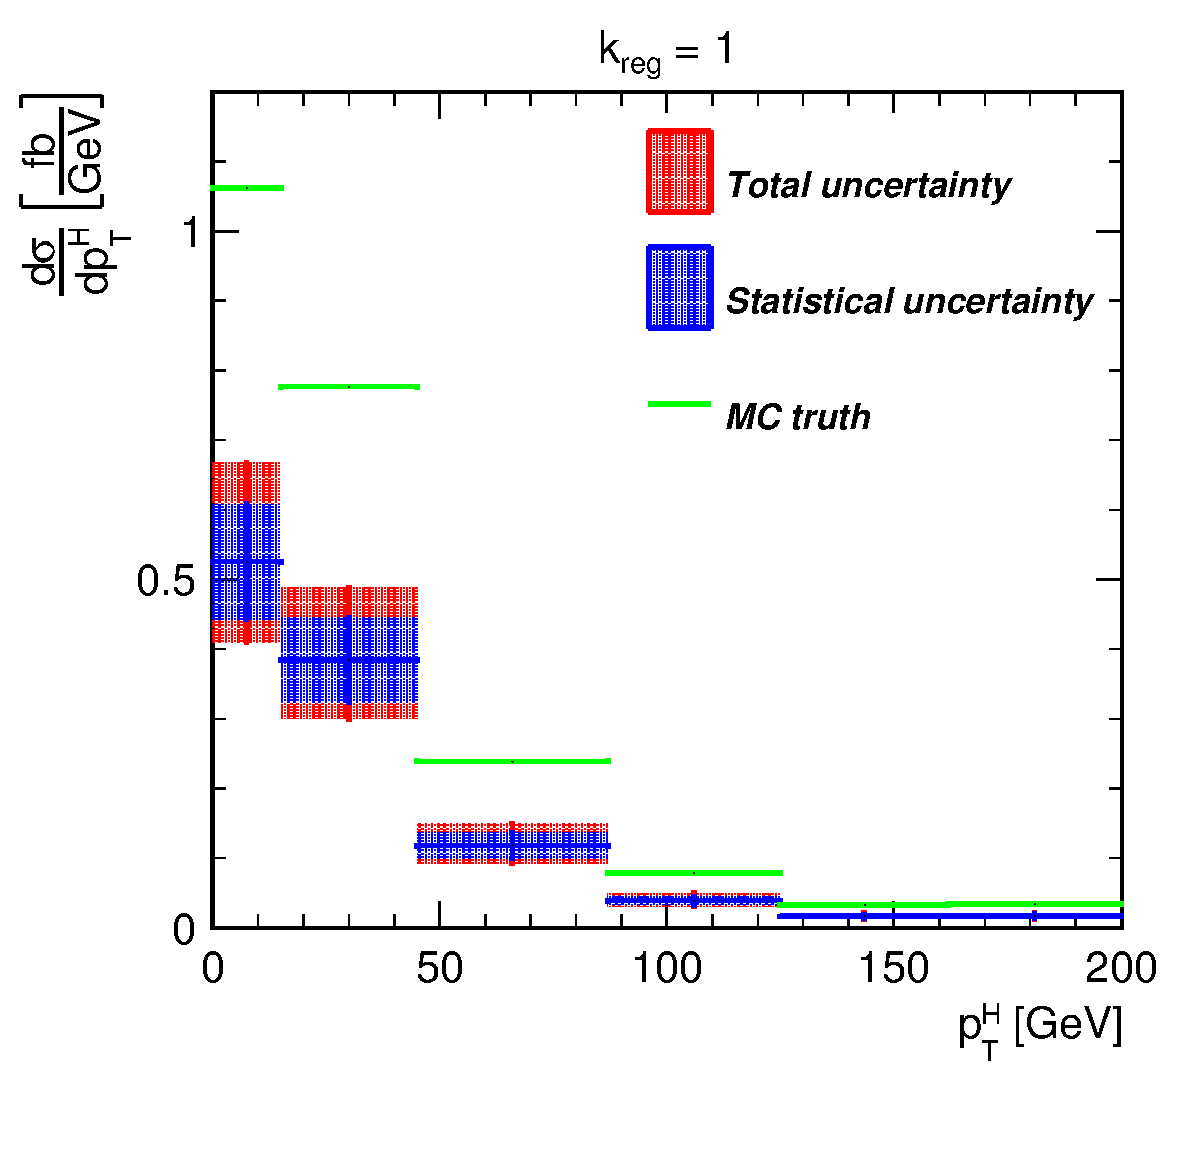
\includegraphics[width=0.45\textwidth]{images/kreg1.pdf}
}
\subfigure{
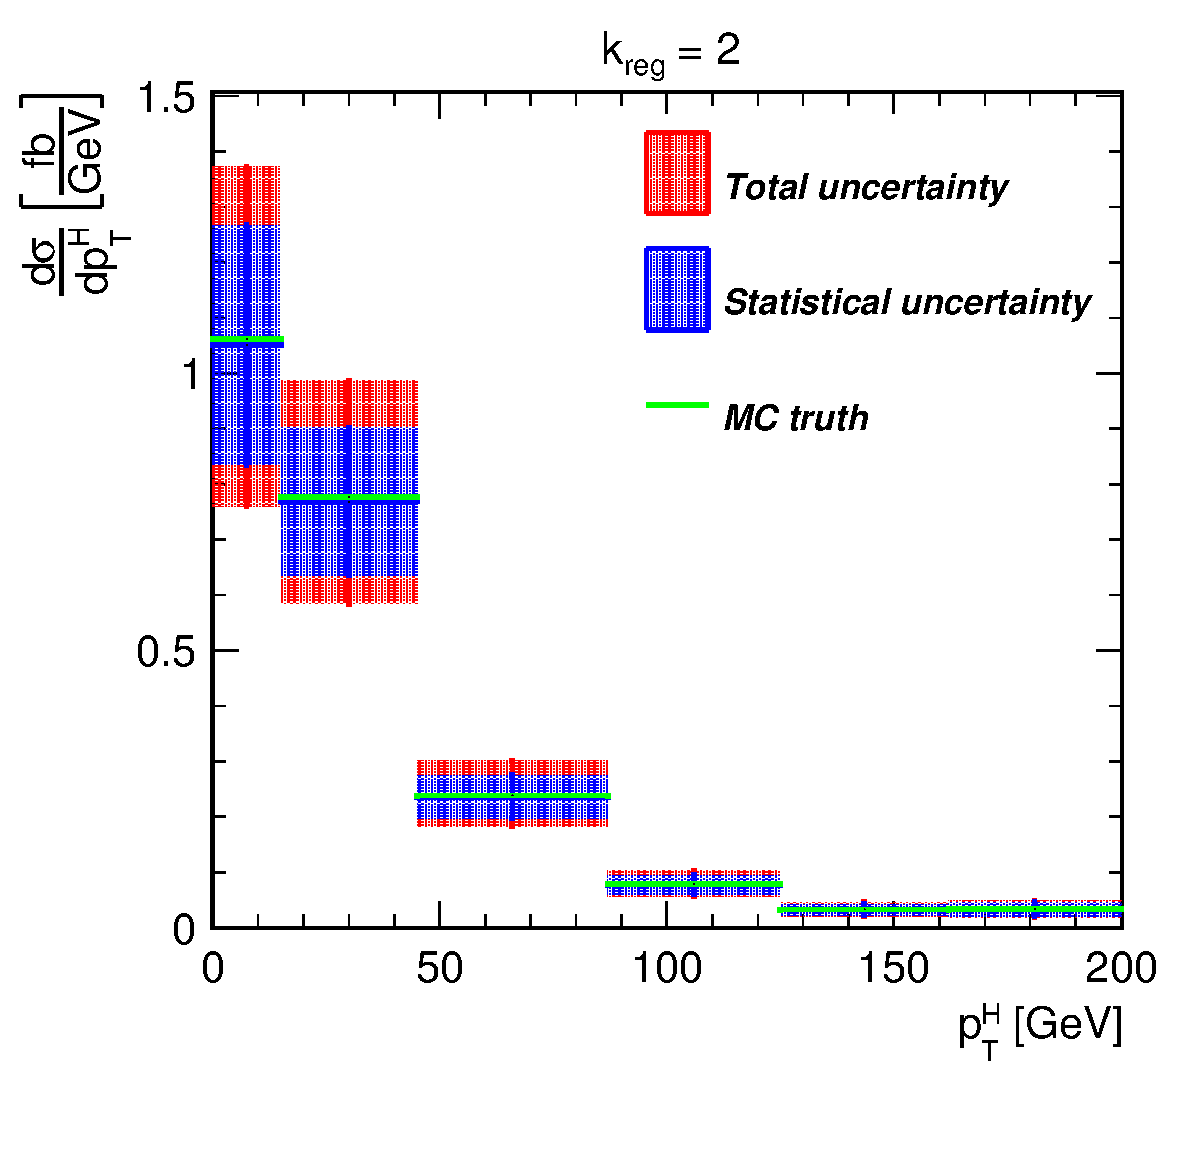
\includegraphics[width=0.45\textwidth]{images/kreg2.pdf}
}\\
\subfigure{
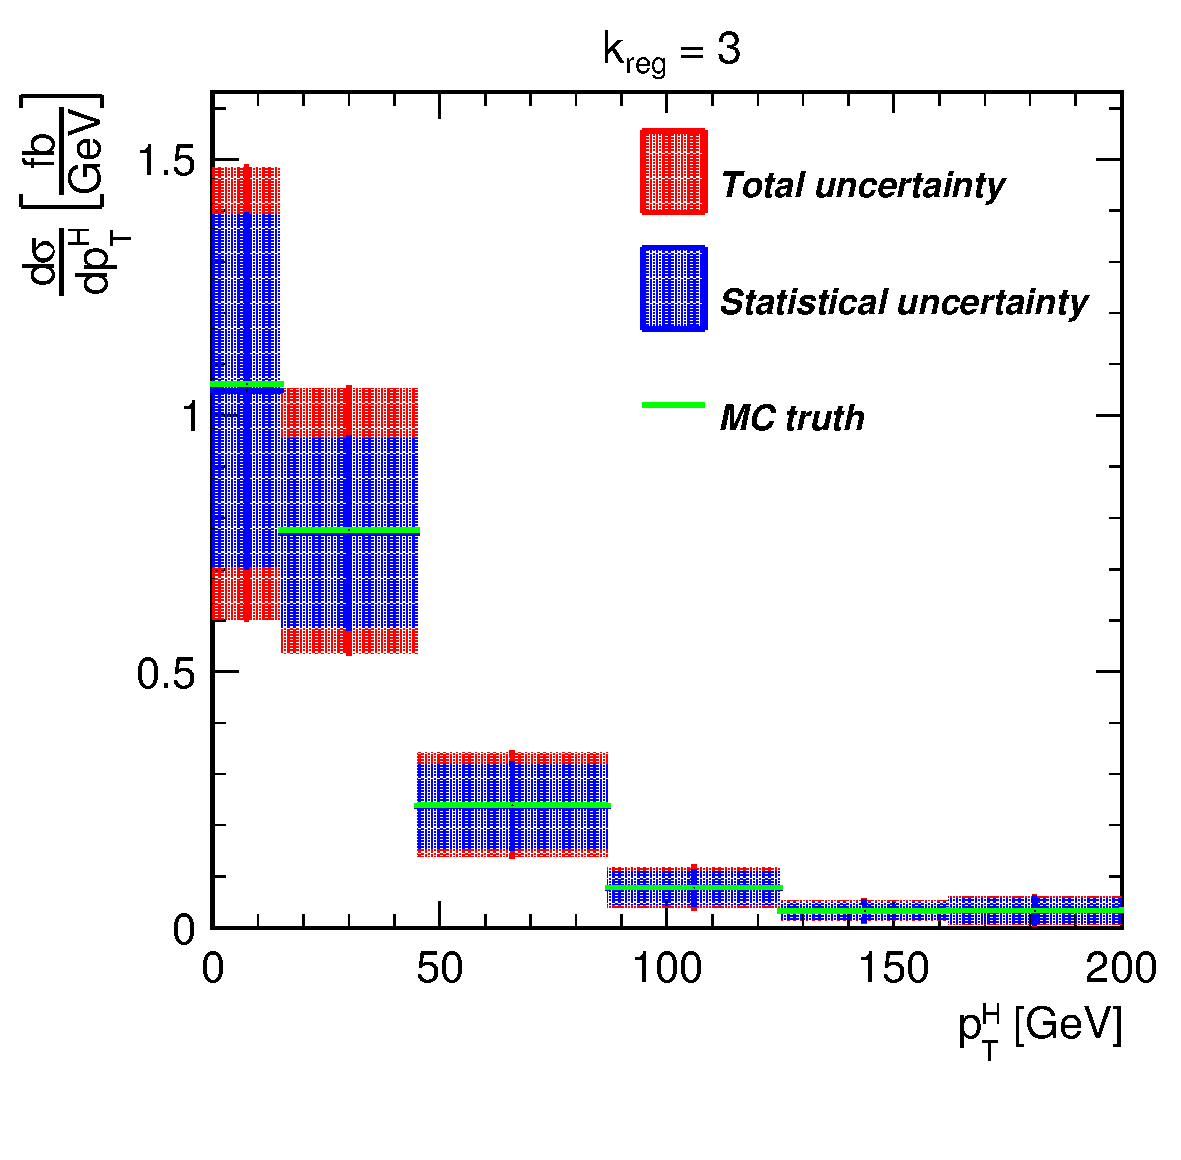
\includegraphics[width=0.45\textwidth]{images/kreg3.pdf}
}
\subfigure{
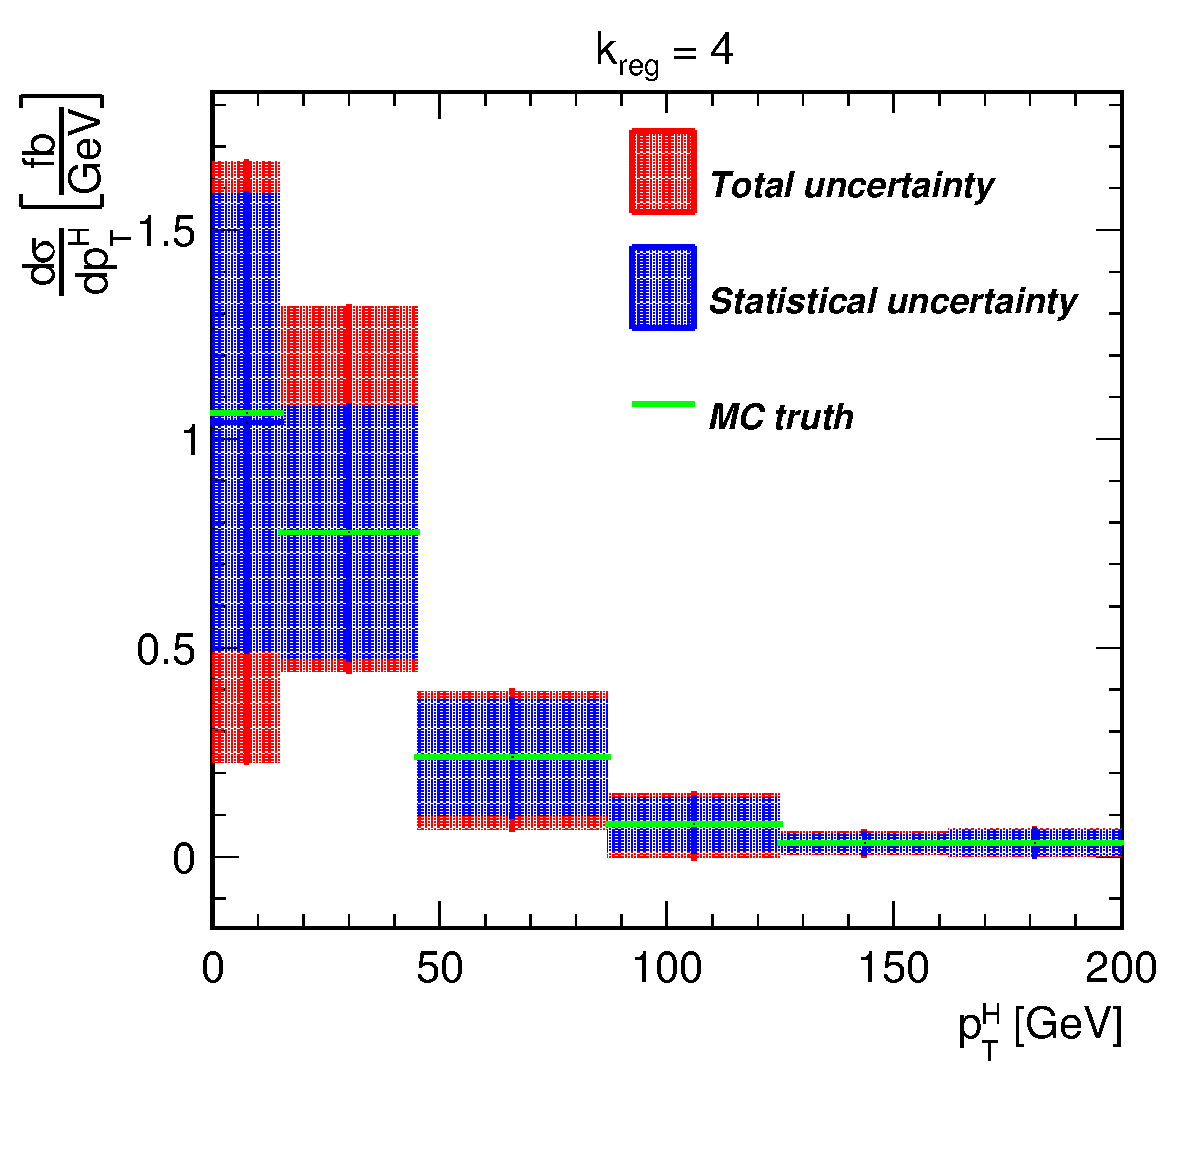
\includegraphics[width=0.45\textwidth]{images/kreg4.pdf}
}\\
\subfigure{
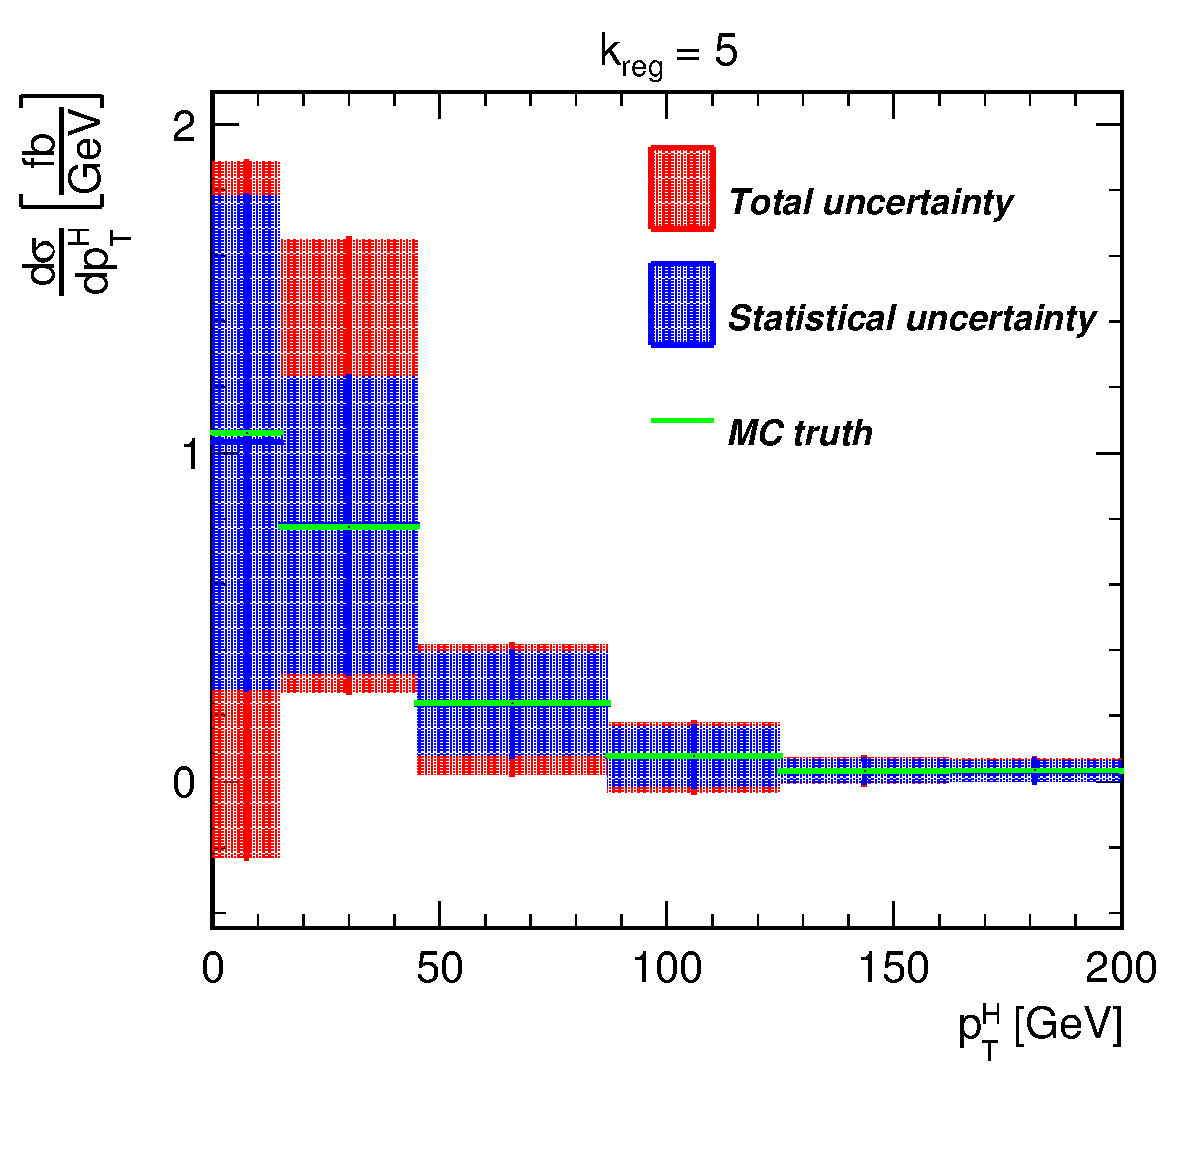
\includegraphics[width=0.45\textwidth]{images/kreg5.pdf}
}
\caption{Unfolded spectrum for several values of the $k_{reg}$ parameter, from 1 (stronger regularization) to 5 (weaker regularization).}
\label{fig:kreg_test}
\end{figure}

Another test that has been performed consists in unfolding a different distribution using the response matrix built with all the signal samples. The different measured distribution used for this test is obtained considering the VBF sample only. The results are shown in figure \ref{fig:VBF_test}, where the unfolded distribution is compared to MC truth, i.e. VBF sample only, for  four different values of the regularization parameter.\\
The plots show that the unfolded spectrum matches the MC truth only for high values of $k_{reg}$, while for lower values the unfolding procedure starts biasing the unfolded distribution, pushing it towards the spectrum used to build the matrix.
Of course this is a very extreme situation, where the measured spectrum is far from the expected one.

\begin{figure}[htb]
\centering
\subfigure[$k_{reg}=2$]{
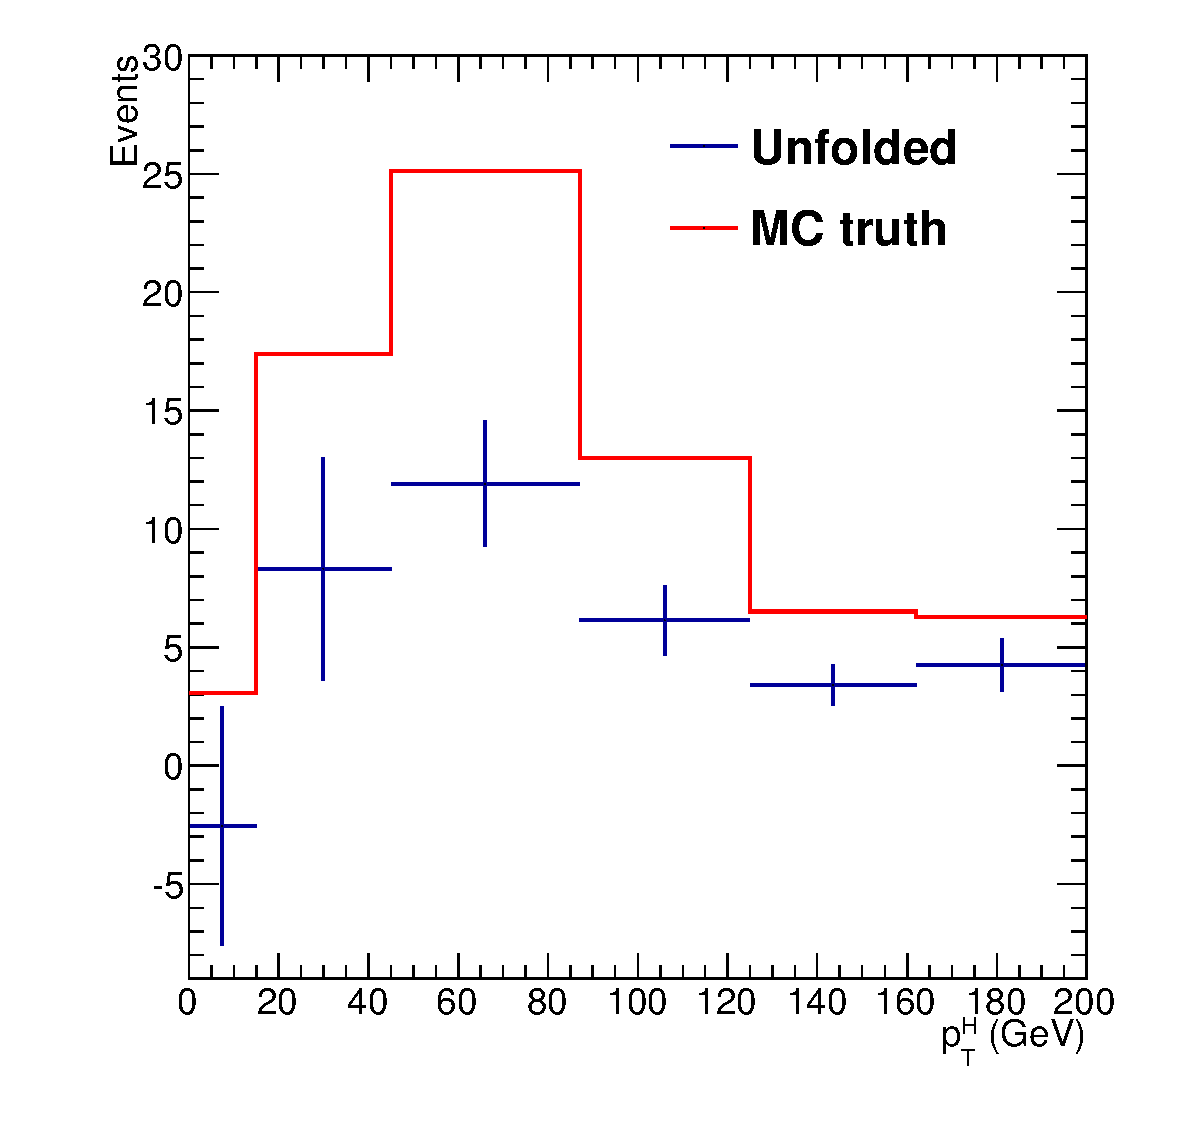
\includegraphics[width=0.45\textwidth]{images/kreg2VBF.pdf}
}
\subfigure[$k_{reg}=3$]{
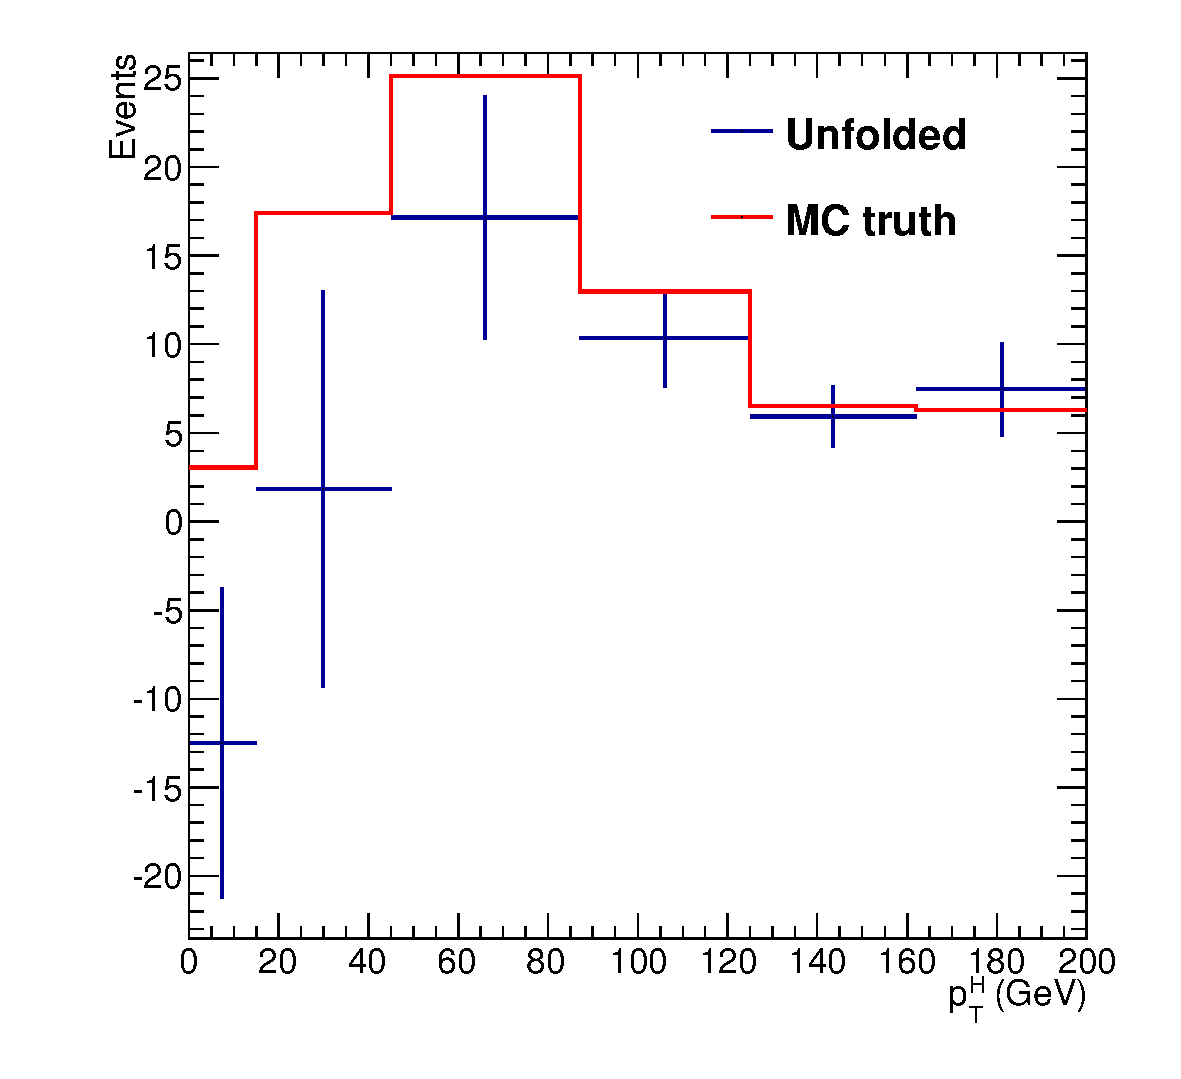
\includegraphics[width=0.47\textwidth]{images/kreg3VBF.pdf}
}\\
\subfigure[$k_{reg}=4$]{
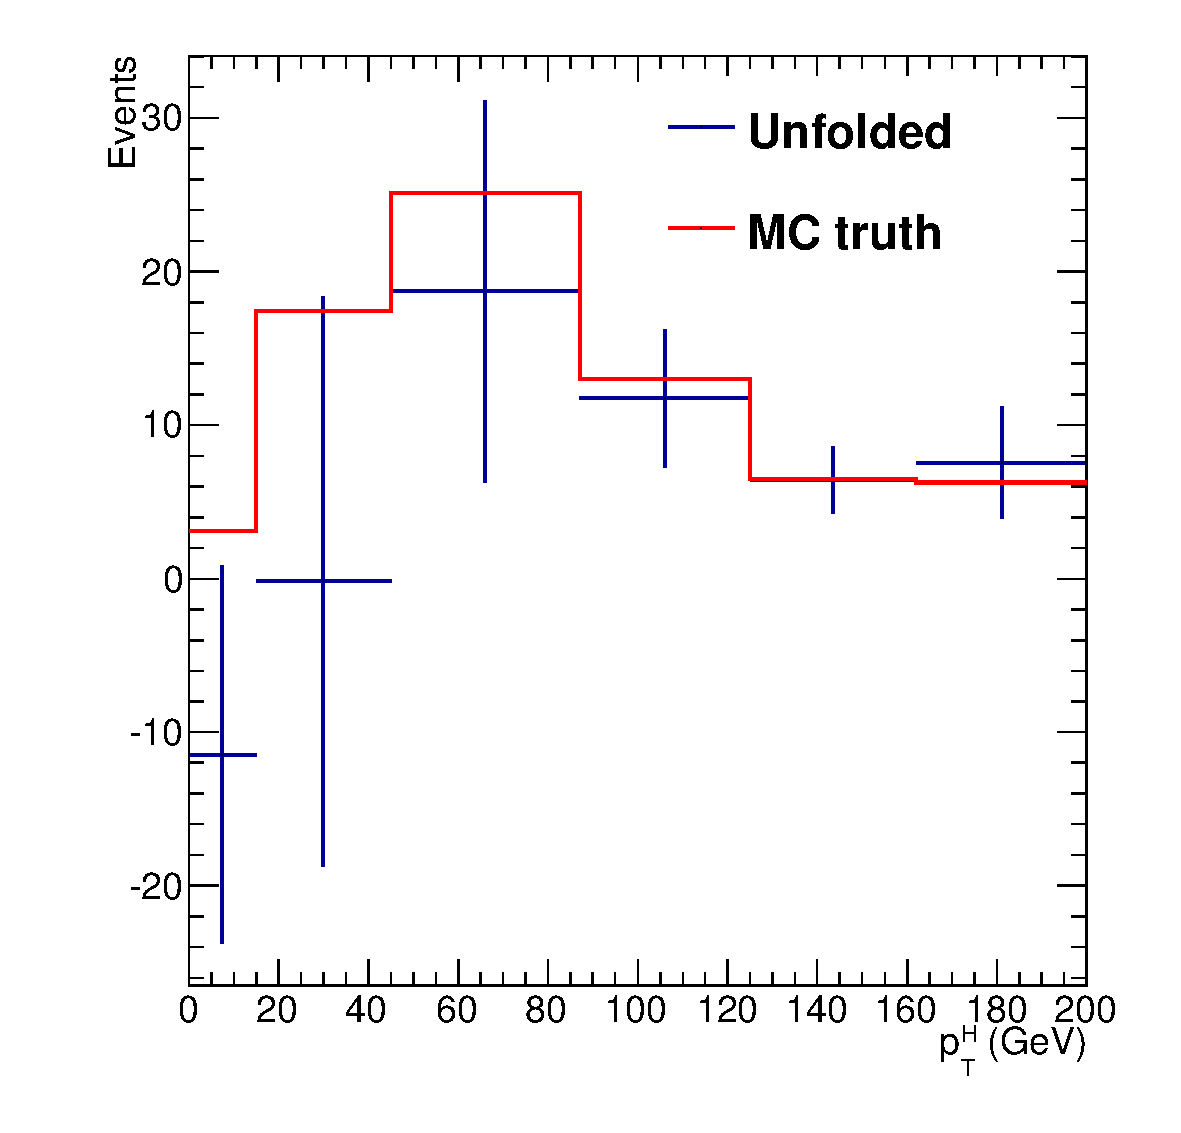
\includegraphics[width=0.45\textwidth]{images/kreg4VBF.pdf}
}
\subfigure[$k_{reg}=5$]{
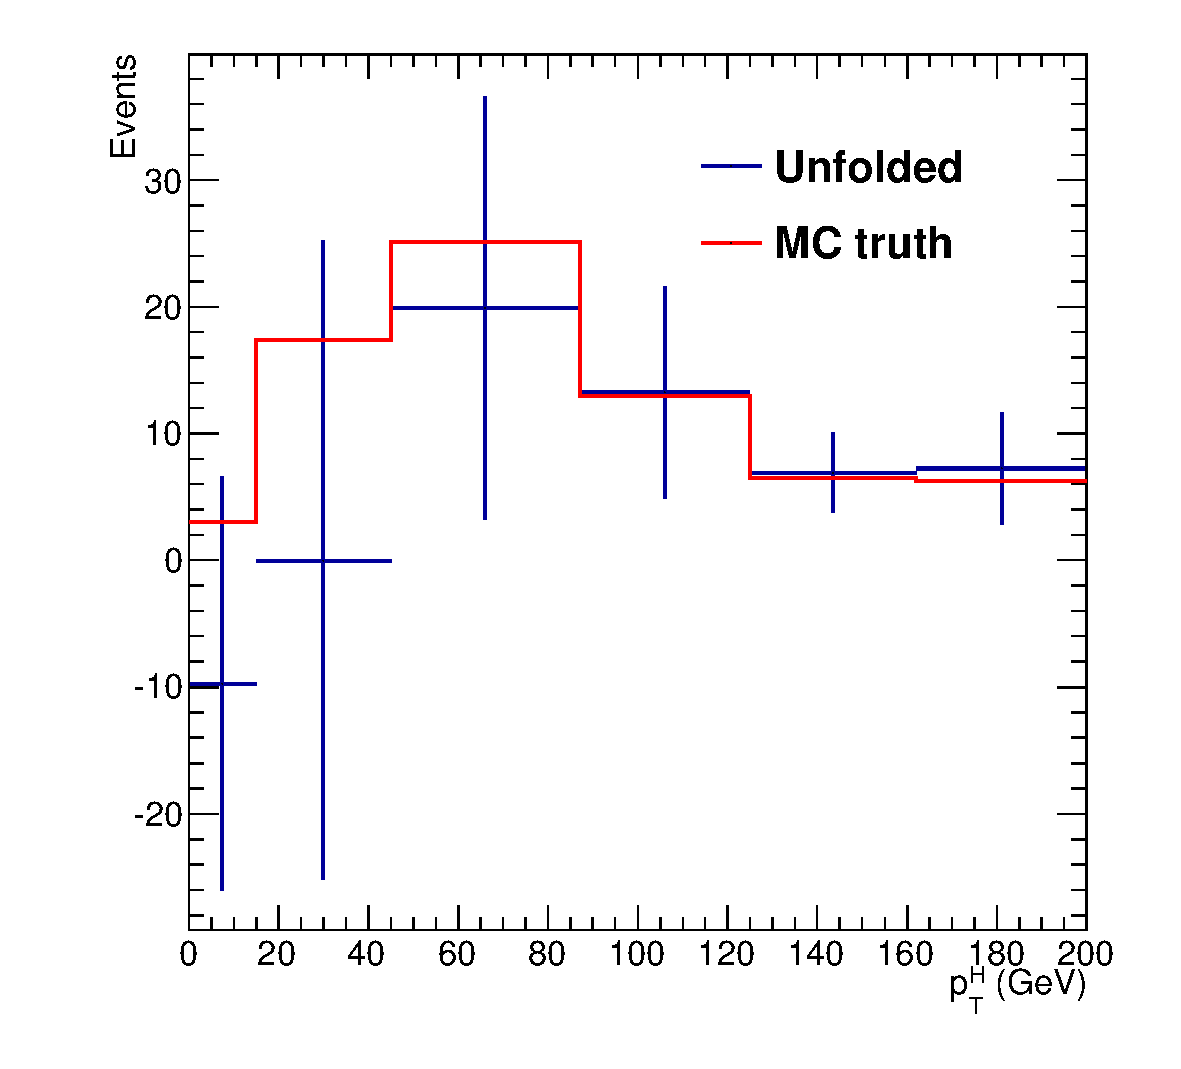
\includegraphics[width=0.47\textwidth]{images/kreg5VBF.pdf}
}
\caption{Unfolded spectrum for several values of the $k_{reg}$ parameter, from 2 (stronger regularization) to 4 (weaker regularization). The response matrix has been applied on top of a measured distribution containing the VBF signal only.}
\label{fig:VBF_test}
\end{figure}



\subsection{Treatment of systematic uncertainties}



